\documentclass[12pt]{article}

\usepackage[french]{babel}
\usepackage[utf8]{inputenc}  
\usepackage[T1]{fontenc}
\usepackage[left=2.5cm,right=2.5cm,top=3cm,bottom=2.65cm]{geometry}
\usepackage{amsmath,amssymb,amsfonts}
\usepackage{algorithm}
\usepackage{algpseudocode}
\usepackage{graphicx}
\usepackage{caption}
\usepackage{tikz}

\graphicspath{{ims/}}

\DeclareMathOperator*{\argmin}{arg\,min}

\newcommand{\Z}{\mathbb{Z}}

\title{
	Computational Geometry and Digital Images\\
	\textbf{Texture Synthesis}\\
	Rapport
}
\author{
	Yoann Coudert-\,-Osmont
	\and
	Jérémy Petithomme
}

\begin{document}
	
\maketitle

\section{Introduction}
	
La synthèse de texture consiste à créer une grande image à partir d'une petite image exemple ou à partir d'un modèle. La texture produite doit respecter une certaine structure mais si elle est produite à partir d'un exemple elle ne doit pas être une simple copie de l'exemple. Nous avons décidé de réaliser un génération de textures à partir d'exemples. \\
Les critères intéressant d'une génération de textures, sont la rapidité d'exécution, la qualité de l'image produite et le contrôle de l'utilisateur. Nous avons décidé d'implémenter un algorithme qui remplie très bien ce dernier critère de contrôlabilité. Nous nous sommes alors penché sur le reproduction du générateur de texture de Lefebvre et Hoppe \cite{Lef++} qui est basé sur la correspondance de voisinages. Ce générateur est parallélisé et peux donc être utilisé en temps réel sur les GPU actuels. Notre implémentation est faite en C++ et est exécuté sur CPU. Les performances sont alors moindres mais le résultat reste satisfaisant.

\subsection{Comment utiliser notre code}

\paragraph{Dépendances}
Certaines installations ont besoin d'être faites :
\begin{itemize}
	\item OpenMp pour la parallélisation. Pour l'installer : \verb|sudo apt install libomp-dev|.
	\item Une partie de la librairie C++ boost pour gérer les fichiers indépendamment du système. Pour l'installer : \verb|sudo apt install libboost-filesystem-dev|.
	\item La librairie C++ GTKmm est utilisée dans notre interface graphique. Pour l'installer : \verb|sudo apt install libgtkmm-3.0-dev|.
\end{itemize}

\paragraph{Le dossier \texttt{ims}}
Dans ce dossier se trouve 3 images et un dossier par images. Les dossiers contiennent des images dites de cohérences qui seront expliqués plus loin. Ces dossiers peuvent aussi contenir des images \verb|res.png| qui sont les résultats obtenus. Pour obtenir plus d'images d'exemples, vous pouvez vous placer dans le dossier \verb|ims| et lancer le script \verb|get_more_images.sh| qui téléchargera d'autres images avec leurs dossiers de cohérences.

\paragraph{Compiler et exécuter}
Nous avons deux exécutables. Le premier peut être créé via la commande \verb|make|. L'exécutable créé a alors le nom \verb|main| et permet d'exécuter notre générateur sur une image et de créer une image pour chaque étape de l'algorithme. Pour l'utiliser, tapez :
\begin{center}
	\texttt{./main <filename> [-c] [-t]}
\end{center}
Le premier argument est obligatoire et est le chemin d'accès à l'image d'exemple (par exemple \verb|ims/1.png|). Les deux paramètres suivants sont optionnels. \verb|-c| permet de calculer les images de cohérences si elle n'existent pas déjà. Si vous voulez les recalculer il faudra supprimer les images de cohérences actuelles. Les images de cohérences sont générés dans un dossier du même nom que l'image d'exemple. L'option \verb|-t| permet de rendre toroïdale l'image donnée en exemple. Il est possible de modifier des paramètres supplémentaires en allant modifiant le début du fichier \verb|mai.cpp|. \\
Le second exécutable est celui de l'interface graphique (\figurename~\ref{gui}). Pour créé cet exécutable il faut utiliser \verb|make g|. Pour lancer alors l'interface graphique il suffit de taper :
\begin{center}
	\verb|./gui [filename]|
\end{center}
Le paramètre \verb|filename| est cette fois-ci optionnelle puisque le fichier peut être chargé dans l'interface graphique. Une fenêtre s'ouvrira et vous aurez à gauche l'image générée et à droite plusieurs sliders permettant de contrôler la texture générée. L'application a tendance a crash. Cela semble venir de l'utilisation de OpenMP avec les threads de Glib. Pour corriger cela il suffit de supprimer \verb|-fopenmp| des flags à la ligne 4 du Makefile puis de recompiler sans oublier de faire \verb|make clean|.

\begin{figure}
	\centering
	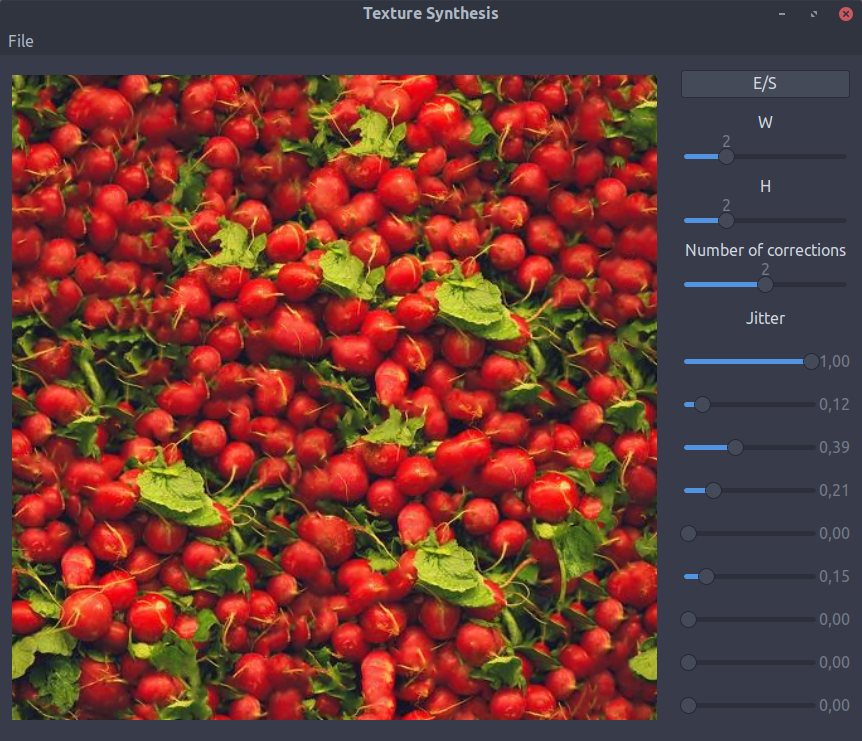
\includegraphics[scale=0.35]{gui.png}
	\captionsetup{justification=centering}
	\caption{GUI qui permet de contrôler la génération et d'avoir le résultat en direct.}
	\label{gui}
\end{figure}

\section{Explication de la méthode de synthèse}

\subsection{Fonctionnement global}

Pour commencer on suppose que l'on part d'une image d'exemple $E$ qui est carrée. Si notre image est rectangulaire alors il suffit de prendre un carré de taille maximale de l'image de départ. On considère donc un exemple $E$ de taille $m \times m$.

\paragraph{Principe générale}

\begin{figure}[t]
	\centering
	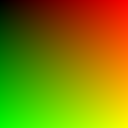
\includegraphics[scale=2.5]{S0.png}
	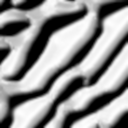
\includegraphics[scale=2.5]{E0.png}
	\qquad \qquad
	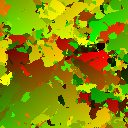
\includegraphics[scale=2.5]{S1.png}
	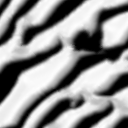
\includegraphics[scale=2.5]{E1.png}
	\captionsetup{justification=centering}
	\caption{Illustration des maps. A gauche la map identité et l'image d'exemple E. A droite une map généré par notre algorithme de synthèse et l'image correspondante $E[S]$.}
	\label{map_illu}
\end{figure}

Le but va être de créer une map $S$, qui à chaque point $p$ du plan $\Z^2$ associe une coordonnée $u$ dans $\{ 0, \dots, m-1 \}^2$ d'un pixel de $E$. La texture générée sera alors $E[S]$, l'image qui à la position $p$, a la couleur $E[S[p]]$. Comme on ne va pas généré une image infini, on restreint $p$ à $\{ 0, \dots, Wm-1 \} \times \{ 0, \dots, Hm-1 \}$ afin de créer une image de taille $Wm \times Hm$. Les coordonnées $u = S[p]$ seront représentées par une image en utilisant les composantes rouge et verte (voir \figurename~\ref{map_illu}).

Pour construire cette map, on va créer une pyramide de map ; les premières map ayant une faible définition $W \times H$ et la dernière une haute définition. La largeur de la texture générée est doublé à chaque étape de la pyramide. On pose alors $L = \lceil \log_2 m \rceil$ le nombre d'étape que l'on réalise et la définition de la dernière image est alors $2^l . W \times 2^l . H$. Une étape est divisé en trois phases. La première est le sur-échantillonnage pour double la taille de la texture. La seconde est une phase de jitter, c'est à dire que l'on rajoute du bruit dans la map. Et la troisième et dernière phase est une correction qui modifie chaque pixel de la map un par un de manière à ce que la nouvelle valeur du pixel colle plus avec son voisinage. La \figurename~\ref{step} illustre une telle étape. On note $S_l$ la map obtenue à l'issue de l'étape $l$. $S_0$ est initialisée par la map qui à tout $p$ dans $\{ 0, \dots W-1 \} \times \{ 0, \dots, H-1 \}$ associe les coordonnées $(0, 0)$. Puis on applique un effet de "Jitter" à $S_0$.

\begin{figure}[t]
	\centering
	\begin{tikzpicture}[>={latex}, very thick]
		\node (S0) at (0, 0) { 
\includegraphics[scale=3]{S0_.png} };
		\node[below of=S0] (E0) { 
\includegraphics[scale=3]{E0_.png} };
		\node[left of=S0] {$S_l$};
		\node[left of=E0] {$E[S_l]$};
		
		\node[right of=S0, node distance=4.25cm] (S1) { 
\includegraphics[scale=3]{S1_.png} };
		\node[below of=S1, node distance=1.8cm] (E1) { 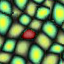
\includegraphics[scale=3]{E1_.png} };
		
		\node[right of=S1, node distance=3.6cm] (S2) { 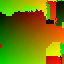
\includegraphics[scale=3]{S2_.png} };
		\node[below of=S2, node distance=1.8cm] (E2) { 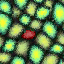
\includegraphics[scale=3]{E2_.png} };
		
		\node[right of=S2, node distance=3.6cm] (S3) { 
\includegraphics[scale=3]{S3_.png} };
		\node[below of=S3, node distance=1.8cm] (E3) { 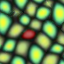
\includegraphics[scale=3]{E3_.png} };
		\node[right of=S3, node distance=1.5cm] {$S_{l+1}$};
		\node[right of=E3, node distance=1.5cm] {$E[S_{l+1}]$};
		
		\draw[->] (S0) -- node[above] {\footnotesize Sur-échantillonage} (S1);
		\draw[->] (S1) -- node[above] {\footnotesize Jitter} (S2);
		\draw[->] (S2) -- node[above] {\footnotesize Correction} (S3);
	\end{tikzpicture}
	\captionsetup{justification=centering}
	\caption{Illustration d'une étape de l'algorithme. Reproduction de la figure 3 de Sylvain Lefebvre et Hugues Hoppe \cite{Lef++}}
	\label{step}
\end{figure}

\paragraph{Calcul de cohérence}

Comme l'image $E_l$ est différente à chaque étape.

\paragraph{Sur-échantillonnage}
Lorsqu'on dispose de $S_{l-1}$, on construit son sur-échantillonnage de la manière suivante :
$$ S_l [2p + \Delta] = \left( S_{l-1} \left[ p \right] + \left\lfloor h_l \left( \Delta - \left( 0.5 \atop 0.5 \right) \right) \right\rfloor \right) \mod m $$
Où $h_l = 2^{L-l}$ est le pas à chaque étape, et $\Delta$ appartient à $\{ 0, 1 \}^2$. Le pas sera en particulier utilisé lors de la phase de correction pour construire les voisinages. Cette formule fait simplement en sorte que chaque pixel $p$ devienne un carré de 4 pixel dont le barycentre des valeurs est $S[p]$.

\paragraph{Jitter}
Pour le jiiter, on se donne une fonction de hachage $\mathcal{H} : \Z^2 \rightarrow [ -1; 1 ]^2$ et un coefficient de jitter $0 \leqslant r_l \leqslant 1$ qui va représenter l'intensité de cette phase. Si $r_l = 0$ alors le jiiter n'a aucune incidence. Voici la modification que l'on réalise sur $S_l$ :
$$ S_l[p] = S_l[p] + \left\lfloor h_l r_l \mathcal{H}(p) + \left( 0.5 \atop 0.5 \right) \right\rfloor $$
Ainsi la modification apporté déplace la coordonnée d'au plus le pas $h_l$. Le jitter est donc de plus en plus fin à chaque étape. La puissance de ce décalage est proportionnelle à $r_l$. Un des grand atout de cet algorithme sera alors la possibilité de contrôle du jitter pour chaque étape.

\paragraph{Correction}
Cette phase est appliquée uniquement pour $l > 2$ afin de ne pas trop corriger le jitter des premières étapes ce qui permet plus de contrôle. Dans cette dernière phase on prend les pixels $p$ un par un et on essaye de modifié $S_l[p]$ de manière à ce que la nouvelle valeur soit plus adéquate avec les valeurs des pixels voisins. Pour cela on considère le voisinage $5 \times 5$ de $p$ dans la texture générée $E_l[S_l]$ :
$$ N_{S_l}^{(5)}(p)_{i, j} = E_l \left[ S_l \left[ p + \left( i \atop j \right) \right] \right] \qquad -2 \leqslant i, j \leqslant 2 $$
Puis pour $u$ dans $\{ 0, \dots m-1 \}^2$, on construit le voisinage de $u$ dans $E_l$ avec un pas de $h_l$ :
$$ N_{E_l}^{(5)}(u)_{i, j} = E_l \left[ u + h_l \left( i \atop j \right) \right] \qquad -2 \leqslant i, j \leqslant 2 $$
A noté que j'utilise la notation $E_l$ et pas $E$. En effet à l'étape $l$ on utilise une image floutée via un filtre gaussien d'écart type $\sigma_l = h_l$. Cette image est donc $E_l$. Cela permet de capturer une information de couleur plus globale comme on calcule un voisinage avec un pas $h_l$. En effet regarder la couleur d'un pixel spécifique à une distance $h_l$ n'as pas de sens lorsque $h_l$ est grand.

Finalement notre but est d'obtenir :
$$ S_l[p] \gets \argmin_{ u \in \{ 0, \dots, m-1 \}^2 } \| N_{S_l}^{(5)}(p) - N_{E_l}^{(5)}(u) \|_2 $$
Mais un algorithme naïf pour faire cela aurait une complexité en $\mathcal{O}(m^4)$ avec un constante multiplicative conséquente puisque l'on calcule des distances dans un espace de dimension 25. Ce n'est pas souhaitable, c'est pourquoi on restreint $u$ à un bien plus petit sous-ensemble de $\{ 0, \dots, m-1 \}^2$.

Pour restreindre l'ensemble des valeurs possibles on remarque dans un premier temps que si on applique pas de jitter on a l'égalité suivante :
$$ S_l[p] = S_l \left[ p + \Delta \right] - h_l \Delta $$
On va donc dans un premier temps reteindre $u$ à l'ensemble des valeurs $S_l \left[ p + \Delta \right] - h_l \Delta$ pour $\Delta$ dans $\{ -1, 0, 1 \}^2$. Pour augmenter la taille de notre sous-ensemble et permettre plus de discontinuités dans notre map, on ajoute le plus proche voisin de chacune de ces valeurs. C'est à dire que l'on pré-calcule une coordonnée $C_1^l(u) \neq u$ tel que $ \| N_{E_l}^{(7)}(u) - N_{E_l}^{(7)}(C_1^l(u)) \|_2 $ est minimale pour chaque $u$. On pose aussi $C_0^l(u) = u$ et on pourrait aussi construire $C_
2^l(u)$ comme étant le second plus proche voisin de $u$. L'ensemble $C^l(u)$ des plus proches voisins de $u$ est appelé ensemble de cohérence de $u$. Dans la pratique on ne calcule que le plus proche voisin car les calculs sont gourmands. On fait aussi en sorte que le plus proche voisin soit éloigné de $u$ dans le sens de la distance $\| u - C_1^l(u) \|_2$ qui ne porte pas sur les voisinages. Enfin pour les petites valeurs de $l$ on calcule pas la distance sur le voisinage $7 \times 7$ mais plutôt sur le voisinage $5 \times 5$ voire $3 \times 3$ si $m$ est faible. On obtient finalement :
$$ S_l[p] \gets C_{i_{\min}}^l \left( S_l \left[ p + \Delta_{\min} \right] - h_l \Delta_{\min} \right) \, , \quad \text{où} $$
$$ i_{\min}, \Delta_{\min} = \argmin_{i = 0, 1 \atop \Delta \in \{ -1, 0, 1 \}^2} \left\| N_{S_l}^{(5)}(p) - N_{E_l}^{(5)} \left( C_i^l \left( S_l[p + \Delta] - h_l \Delta \right) \right) \right\|_2 \varphi(i) $$
Où $\varphi(i)$ est un terme qui permet de pénaliser le changement pour donner une priorité à la continuité dans la texture générée. Ce terme vaut $1$ pour $i = 0$ et est strictement plus grand que 1 pour $i > 1$.

Pour la mise à jour de $S_l$ durant la correction on utilise les sous-passes décrites en 3.3 de l'article \cite{Lef++}. Les sous-dossiers dans le dossier \verb|ims| contiennent les images de cohérence pour chaque étape. Les calculs des plus proches voisins sont exacte et le temps d'exécution est alors long (environs 8 / 10 minutes). Une amélioration possible serait alors de faire une recherche approchée du plus proche voisin \cite{Ary++}.

\subsection{Embellissement de l'image finale}

\paragraph{Pour les grands}

Si l'image d'exemple est trop grande le temps de calcul risque d'être long. On divise alors la largeur par $2^p$ avec $p$ choisi de manière à obtenir une nouvelle image de largeur comprise entre 129 et 256. Nous avons commencé par réduire la taille en faisant un filtrage gaussien puis en prenant le premier pixel de chaque bloc de largeur $2^p$ mais le résultat n'était pas au rendez vous. Nous sommes revenu sur quelque chose de plus simple en prenant la valeur moyenne sur chaque bloc de largeur $2^p$. On note $E_l$ l'image réduite et $E_h$ l'image de départ.

Une fois que notre algorithme a produit la map $S_l$ pointant vers les pixels de $E_l$, on construit une nouvelle image $I$ de meilleure qualité en faisant une interpolation. Voici le calcul effectué pour trouvé la nouvelle couleur du pixel à la position $(x, y)$ via la fonction \textsc{Magnify} (Algorithm \ref{alg:magn}). La \figurename~\ref{magn_res} montre le résultat obtenu en appliquant cette fonction.

\begin{algorithm}
	\caption{Amélioration de la qualité}
	\label{alg:magn}
	\begin{algorithmic}
		\Function{Magnify}{$x, y$}
			\State $x_L, \, y_L \gets x / 2^p, \, y / 2^p$
			\State $dp = (dp_x, dp_y) \gets x \mod 2^p, \, y \mod 2^p$
			\For{$i, j \in \{ 0, 1 \}^2$}
				\State $u_{i, j} \gets 2^p \left( S \left[ x_L + i, \, y_L + j \right] - \left( i, \, j \right) \right) + dp$
				\State $color \left[ i, \, j \right] \gets E_h \left[ u_{i, j} \right]$
			\EndFor
			\State \Return $color \left[ 0, \, 0 \right] (1 - dp_x) (1 - dp_y)
						+ color \left[ 1, \, 0 \right] dp_x (1 - dp_y)$
			\State $\qquad \qquad + \, color \left[ 0, \, 1 \right] (1 - dp_x) dp_y
						+ color \left[ 1, \, 1 \right] dp_x dp_y$
		\EndFunction
	\end{algorithmic}
\end{algorithm}

\begin{figure}[h]
	\centering
	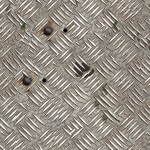
\includegraphics[scale=3.2]{downsized.png} \qquad \quad
	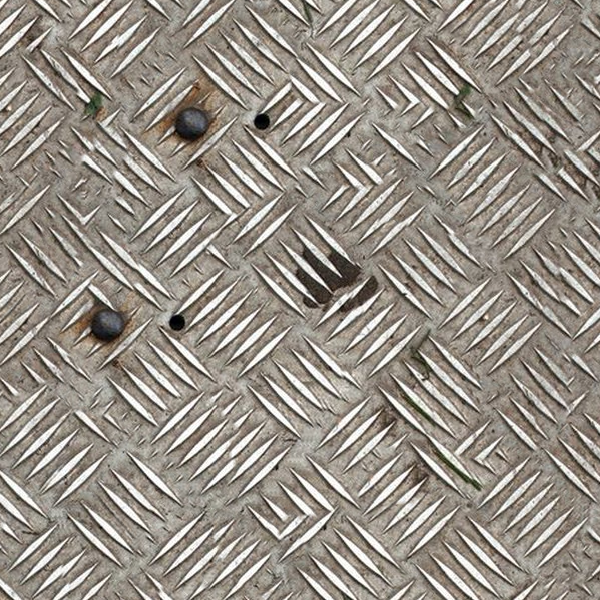
\includegraphics[scale=0.8]{magnific.png}
	\captionsetup{justification=centering}
	\caption{A gauche l'image synthétisé avec l'exemple de faible qualité $E_L$ et à droite l'image obtenue après application de l'algorithme pour augmenter la qualité.}
	\label{magn_res}
\end{figure}

\paragraph{Et les petits}
Pour les images dont la taille n'est pas trop grande on rencontre un autre problème qui est la visibilité accrue des bordures entre les zones continues de la map. On peut voire dans pas mal de cas une séparation assez net. Pour corriger cela on applique un filtre moyennant sur ces bordures (\figurename~\ref{petit}). Un pixel $p$ est sur une bordure si de ses 4 voisins $p'$ vérifie $\| S_L[p] - S_L[p'] \|_1 > 4$.

\begin{figure}
	\centering
	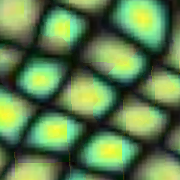
\includegraphics[scale=3]{bordure.png}
	\quad
	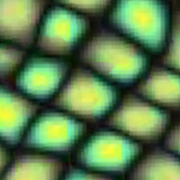
\includegraphics[scale=3]{flou.png}
	\captionsetup{justification=centering}
	\caption{A gauche l'image synthétisé et à droite le résultat obtenue après floutage des bordures.}
	\label{petit}
\end{figure}

\section{Résultats}

\paragraph{Temps d'exécution}
Chez moi le temps d'exécution pour quadruplé la taille de \verb|ims/1.png| est de 2.2s en utilisant la parallélisation d'OpenMp avec un processeur à 4 cœurs. Sans OpenMP j'obtiens un temps d'exécution de 5.4s. La parallélisation apporte beaucoup et on peut imaginer que les performances doivent être très bonnes sur un GPU.

\paragraph{Qualité}
La qualité de la texture générée est souvent très bonne quand l'image d'exemple ne contient pas de structure très carré et à grande échelle. La page suivante présente dans un premier temps des exemples qui fonctionnent plutôt bien (\figurename~\ref{good}). En revanche les résultats sont assez mauvais sur des images qui ont une structure stricte et bien définie comme des legos ou du texte.

\begin{figure}[p]
	\centering
	\begin{tikzpicture}
		\node (z0) at (0, 0) {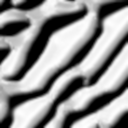
\includegraphics[scale=2.3]{E0.png}};
		\node[right of=z0, node distance=5cm] {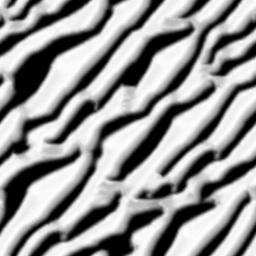
\includegraphics[scale=0.57]{zebre.png}};
		
		\node[below of=z0, node distance=5.4cm] (l0) {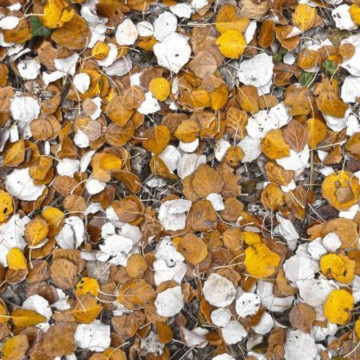
\includegraphics[scale=0.85]{leaf0.jpg}};
		\node[right of=l0, node distance=5cm] {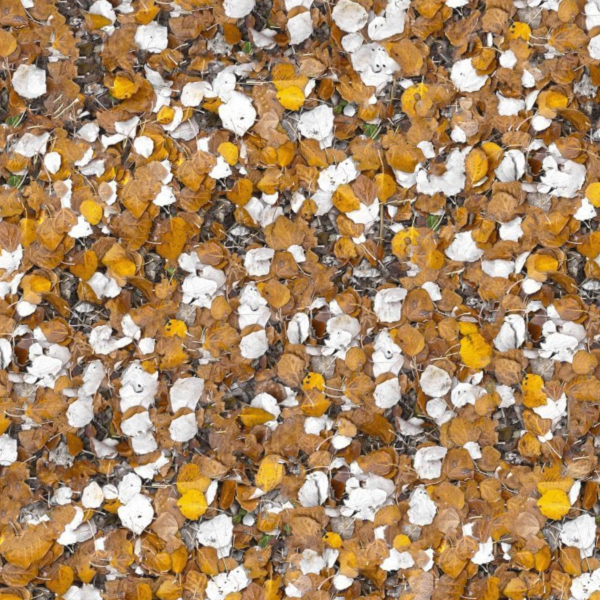
\includegraphics[scale=1.02]{leaf1.png}};
		
		\node[below of=l0, node distance=5.4cm] (v0) {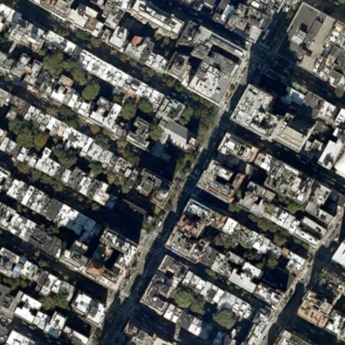
\includegraphics[scale=0.22]{ville0.jpg}};
		\node[right of=v0, node distance=5cm] {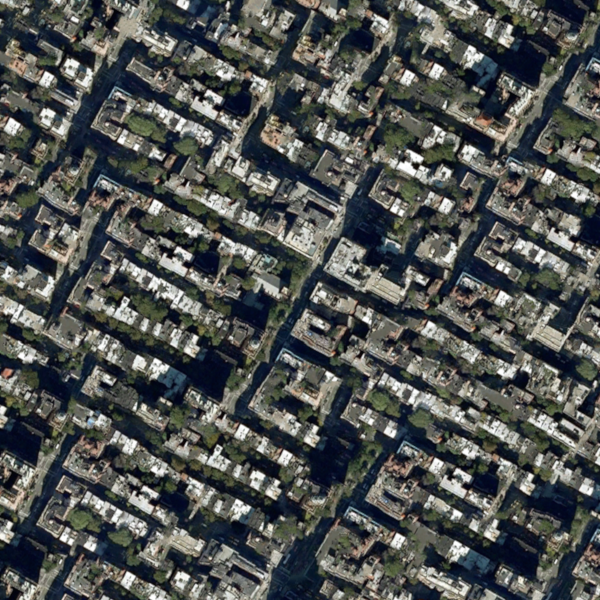
\includegraphics[scale=1.02]{ville1.png}};
		
		\node[below of=v0, node distance=5.4cm] (o0) {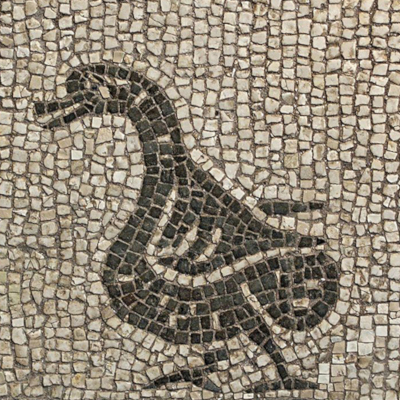
\includegraphics[scale=0.84]{oie0.jpg}};
		\node[right of=o0, node distance=5cm] {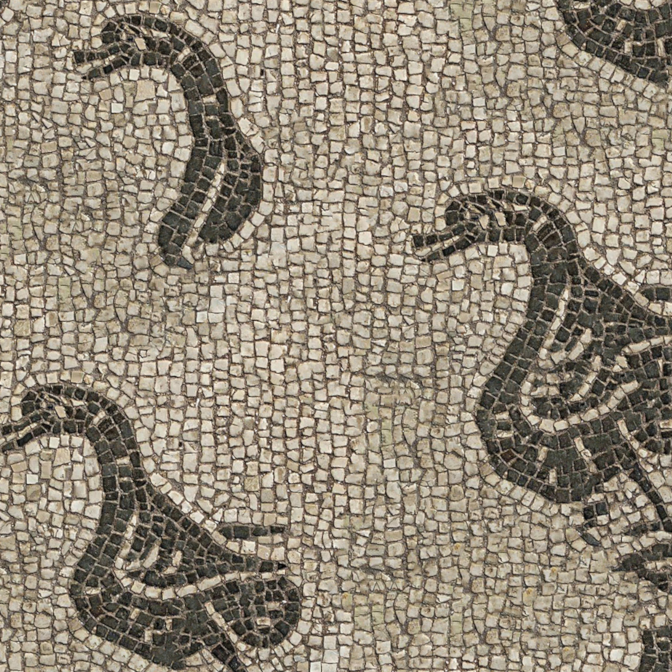
\includegraphics[scale=0.92]{oie1.png}};
	\end{tikzpicture}
	\captionsetup{justification=centering}
	\caption{Exemples qui fonctionnent assez bien. Pas de structure très carré.}
	\label{good}
\end{figure}

\begin{figure}[p]
	\centering
	\begin{tikzpicture}
		\node (t0) at (0, 0) {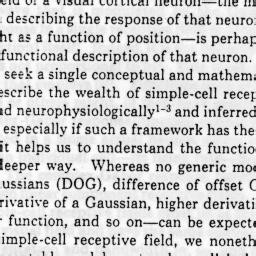
\includegraphics[scale=0.055]{text0.jpg}};
		\node[right of=t0, node distance=7cm] {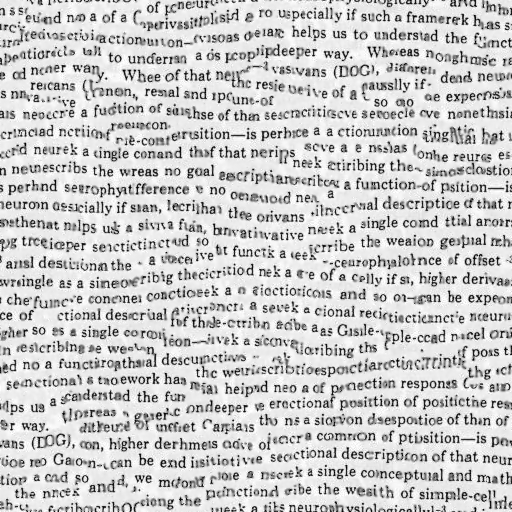
\includegraphics[scale=0.42]{text1.png}};
		
		\node[below of=t0, node distance=8.6cm] (l0) {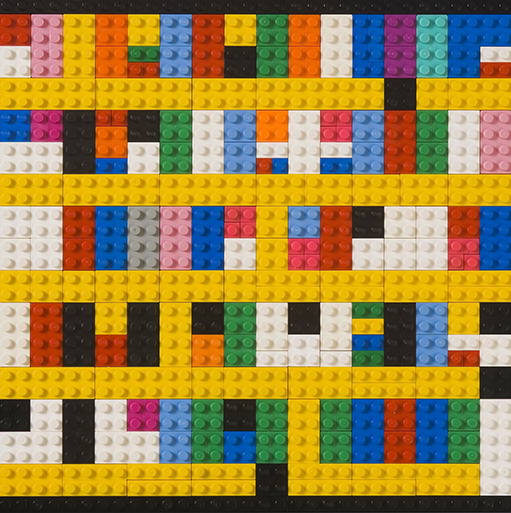
\includegraphics[scale=0.2]{lego0.jpg}};
		\node[right of=l0, node distance=7cm] {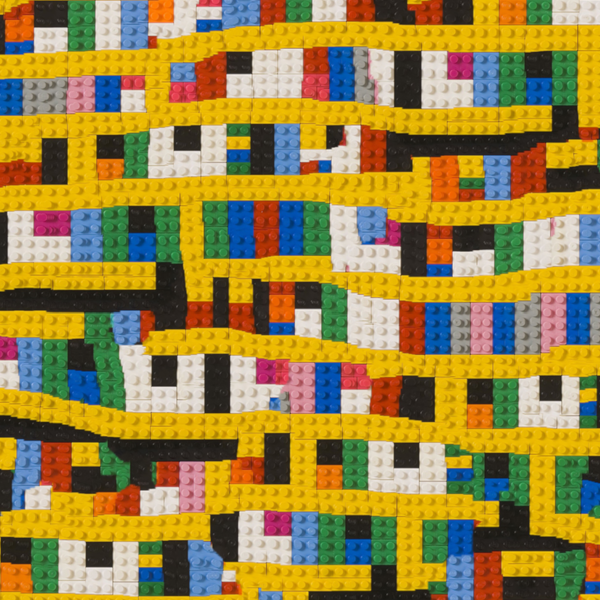
\includegraphics[scale=1.5]{lego1.png}};
	\end{tikzpicture}
	\captionsetup{justification=centering}
	\caption{Exemples qui échouent. Les logos et le texte ont une structure très carré/précise que la générateur de texture n'arrive pas à reproduire.}
	\label{bad}
\end{figure}

\appendix

\bibliographystyle{plain}
\bibliography{bib.bib}


\end{document}